\documentclass{article}
\usepackage{multicol}
\usepackage{graphicx}
\usepackage[top=1.03in, bottom=0.51in, left=0.93in, right=0.92in]{geometry}

\usepackage{color}
\usepackage{url}
\usepackage{hyperref}
\definecolor{linkcolour}{rgb}{0,0.2,0.6} 
\hypersetup{colorlinks,breaklinks,urlcolor=linkcolour, linkcolor=linkcolour}  
\usepackage{pdfpages}

%wrapfig
\usepackage{wrapfig}
\usepackage{lipsum}  % generates filler text

\renewcommand{\familydefault}{\sfdefault} 

\renewcommand{\labelenumi}{\Roman{enumi}. }

\begin{document}
\definecolor{orange}{rgb}{0.9648,0.4960,0}

\begin{figure}[ht]
\begin{minipage}[t]{0.40\linewidth}
\centering
\raisebox{-\height}{
\includegraphics[width=2in]{UT-logo2.png}}

\label{fig:figure1}
\end{minipage}
\hspace{0.5cm}
\begin{minipage}[t]{0.5\linewidth}
\centering 
\vskip 0.2cm
\textcolor{orange}{\huge \bf CASE STUDY}
\vskip 0.2cm 
{\Large \bf Modeling and Simulation}
\vskip 0.2cm 
{\Large \bf Dr. Xueping Li }

\end{minipage}
\end{figure}
{\bf
\begin{tabular}{ll}
%Course Section:	& IE 526 \\
\textcolor{orange}{------------------------------------------------------------------------------------------------------------------------------}
\end{tabular}
}

%%\vskip 0.3in

\begin{center}
{\textcolor{orange}{ \bf Case Study: Serial Process v.s. Parallel Processing(\#2)}}
\end{center}
\vskip 0.2in

%\begin{enumerate}

%\item 

\textcolor{orange}{\bf Goal::} \textit{To learn the following methods/techniques:}\\
\begin{itemize}
\item Process Modeling Library: source, queue, delay, sink, select output, time measure start/end etc.
\item Define variables and display its value.
\item Collect statistics such as Time in System (TIS), Average Waiting Time in Queue (AWTQ), Time Average Number of parts in Queue (TANQ), Working in Process (WIP), utilization, etc.
Use Time Measure Start/End to collect TIS/AWTQ and display a histogram. Use Statistics to collect discrete/continuous performance measures. 
\item Make plots such as histogram plot, time plot, etc.
\item Basic animation: status of the machine, queue, delay, etc. through Space Markups. 
\item Define Agent (Entity) Type and attributes. Collect TIS through this method. Collect ``exact'' statistics for Time Average of WIP and Average TIS. 
\item Introduce ``Service'' and ``Resources''.
\item Add logo/images to ``Simulation'' window.
\item ``Split'' module \& use of ``Dataset''. 
\item ``Multiple runs/replicates'' through ``Parameter Variation''. 
\item Export/Import data to text files/Excel/database et al.
\item Assist business decision-making based on simulation models.
\end{itemize}


\vskip 0.3in

\textcolor{orange}{\bf Problem Statement:}  ABC Firm provides financial products to customers. In this study, we investigate the ``loan application'' process. People (``applicants'')
arrive to the firm with exponential interarrival times with a mean 1.25 hours. Each application has to go through 4 steps: check credit, prepare the contract, price the loan, and disburse the funds.
Each of the 4 steps take about 1 hour which assumes to follow the exponential distribution.  \\

There are four employees in the firm, namely Alfie, Betty, Chuck, and Doris. Each is able to process any of the work in the above 4 steps. We have two systems, ``System 1'' and ``System 2''. See  figures \ref{fig:sp} and \ref{fig:pp}.

\begin{figure}[htbp]
\begin{center}
	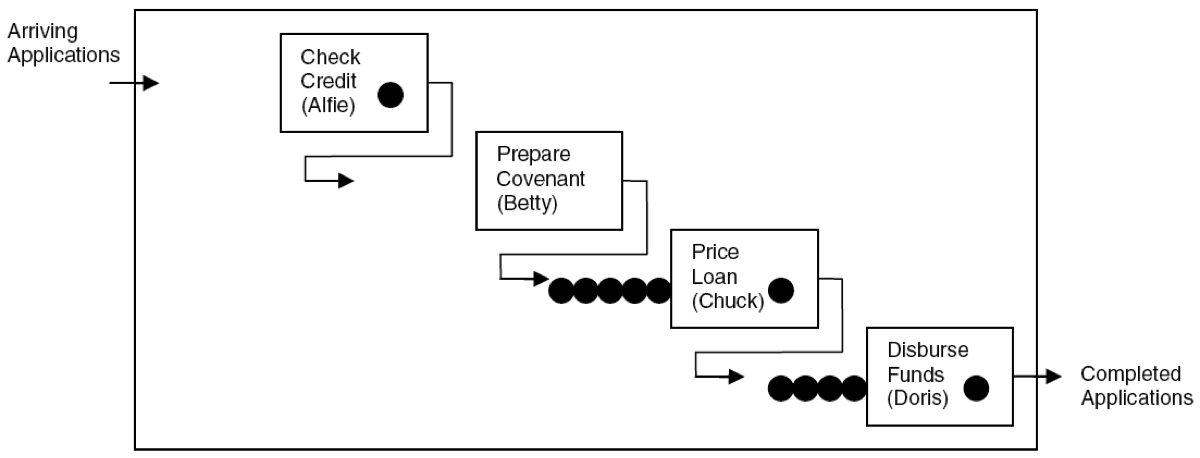
\includegraphics [width=0.66\textwidth] {SP.png}
\caption{``System 1'': Serial Processing}
\label{fig:sp}
\end{center}
\end{figure}

\begin{figure}[htbp]
\begin{center}
	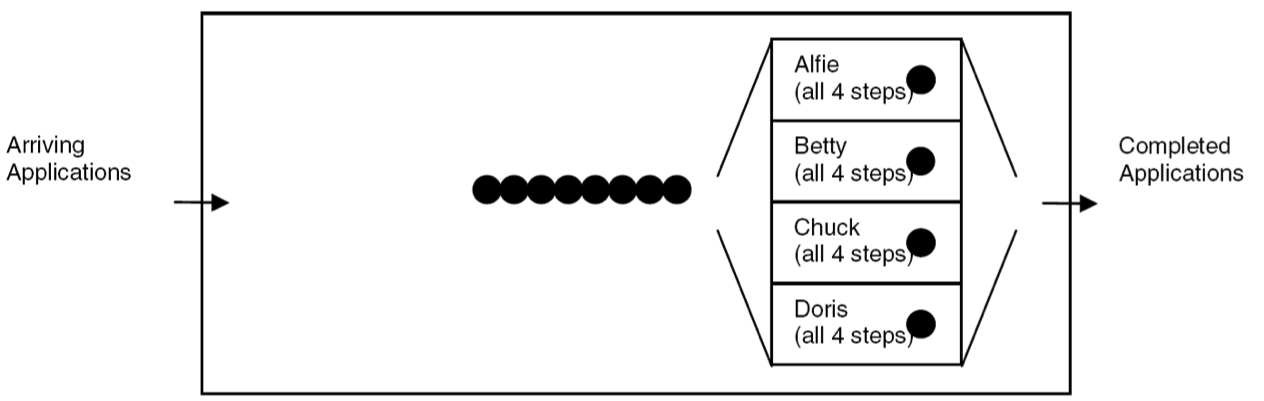
\includegraphics [width=0.66\textwidth] {PP.png}
\caption{``System 2'': Parallel Processing}
\label{fig:pp}
\end{center}
\end{figure}

\vskip 0.3in

So, the question is, which system do you recommend to Mr. Big Boss of the ABC Firm? ``System 1'' or ``System 2''? Why? \textit{A tip}: Mr. Boss is interested in the average, and maximum number
of applications in the process (WIP) and he is also interested in the average and maximum time in system of the applications.  

\vskip 0.3in
Build a model and run 160 hours (assuming 7/24/365).

\vskip 0.3in
\textcolor{orange}{\bf Other thoughts:} How to make a fair side by side comparison of the two systems? [\texttt{Spoiler: Clone/Split module}] Show summarized results along with plots. How to make multiple runs? How many runs are needed to make decisions/recommendations? 
\vskip 0.3in

\textcolor{orange}{\bf Handout Companion:} Screencasts will be provided, along with ``multiple runs'' handouts.  


\end{document}

